\newpage
\section*{\hfil ВВЕДЕНИЕ \hfil}
	В современной добыче полезных ископаемых активно применяются средства математического моделирования для симуляции процессов, происходящих в пласте. Однако, на данный момент полноценное моделирование не представляется возможным, поэтому используются различные приближенные методы. Для правильной симуляции процессов, происходящих в недрах, необходимо смоделировать саму среду, в которой эти процессы протекают. Обычно, данные о структуре среды доступны только в некотором количестве точек(скважин), в которых непосредственно идет добыча. Предлагается попытаться использовать методы машинного обучения для синтеза модели среды, похожей на природную. В рамках решения этой проблемы возникает задача синтеза текстур с трендами, например, для учета каких-либо межскважинных корреляций. 
	
	Под текстурой с трендом в данном случае понимается изображение, в котором есть изменение некоторой статистической характеристики вдоль одного из направлений. Такими характеристиками, например, могут быть изменение интенсивности появления частиц среды или пористости среды.
	
	Базовым подходом в задаче синтеза текстур на данный момент является использование искусственных нейросетей. Однако, известные работы в области синтеза текстур с помощью искусственных нейросетей \cite{texture-synthesis-using-CNN, texture-networks} показывают, что у нейросетевых моделей есть проблемы с воспроизведением формы объектов, а также различных пространственно скоррелированных структур. Соответсвенно, целью данной работы ставится поиск нейросетевой архитектуры, способной улавливать и воспроизводить протяженные корреляции.
	
	Для упрощения задачи, будем в дальнейшем рассматривать множество изображений с трендами, удовлетворяющее следующим ограничениям:
	
	\begin{itemize}
		\item Это монохромные изображения 256 x 256 пикселей
		\item Изменяющимся свойством является интенсивность появления частиц $\lambda$
		\item Тренд является линейным и направлен вдоль оси изображения $z_1$: 
		$ \lambda = \lambda_{init} + k z_1 $
	\end{itemize}
	
	Каждый такой тренд фиксируется, соответственно, значениями $\lambda_{init}$ и $\lambda_{final}$. Пример подобного изображения с трендом приведен на (Рис. \ref{1-trend-example}):
	
	\begin{figure}[h]
		\centering{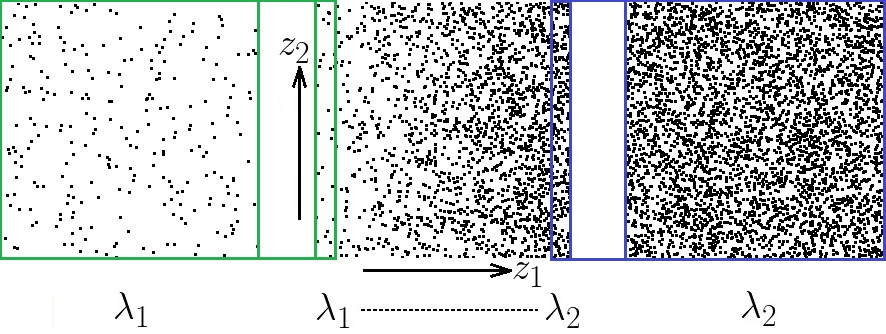
\includegraphics[width=\linewidth]{1-introduction/trend-example}}
		\caption{Пример изображения с трендом, фиксируемого двумя изображениями}
		\label{1-trend-example}
	\end{figure}